\chapter{The geometry of the SVD}

The human eyes and brain are a marvelous system for processing visual information. We can use this to our advantage when studying the \svdp. There are many ways to approach the SVD and a few are explored in this book. One way which may be the favorite for a significant proportion of readers is the geometric approach of this chapter which relies heavily on visual presentation.

Part of the approach so far has relied on imagery to help convey the message. Block diagrams are used to prevent basic shape and size information. The null space vectors in the domain matrices are shaded. The sabot matrix is blocked using a horizontal and a vertical line. The goal is to foster visualization and to use imagination as a adjunct to memorization. 

We can extend the visualization to the area of greatest impact: the geometry of the SVD. In here we will ``see'' the singular values and how they are dilation factors. We will ``see'' how matrices act upon vectors. We will ``see'' how the domain matrices can be represented as rotation matrices, permutation matrices and their compositions. We will ``see''the collapse vector spaces onto lower dimensional objects. Hopefully, this will conjure a perception that the SVD is a geometric process as much as an algebraic process.
 
%%
\section{The geometry of the SVD}
The geometry of the \svdl \ provides helpful insights into many problems. We will see the a marvelous depiction of the conditioning to a system. We will also see a clear depiction of the singular values as scale factors.

%%
\subsection{The image of a matrix}
A matrix acts on a vector and produces another vector. Looking at this action on unit vectors is helpful. Consider the locus of all possible unit vectors -  the unit circle. The unit vectors are parameterized as
\begin{equation}
  x_{\theta} = \mat{c}{\cos \theta \\ \sin \theta}, \quad \theta\in[0,2\pi).
\end{equation}

Figure \eqref{fig:maps:both} below shows two plots. The unit circle is the plot of $x_{\theta}$ as $\theta$ varies from 0 to 2$\pi$. The ellipse is the vector showing the action of the target matrix on the unit vectors:
\begin{equation}
  y_{\theta} = \A{}x_{\theta} = \mat{r}{\cos \theta + 2\sin \theta\\-\cos \theta + 2\sin \theta}. 
\end{equation}

The ellipse represents the ``image'' of the target matrix; the action of the matrix on the unit vectors. The context here is a graphical representation. Later we will see this word used in the context of vector space. 

\begin{figure}[htbp] %  figure placement: here, top, bottom, or page
   \centering
   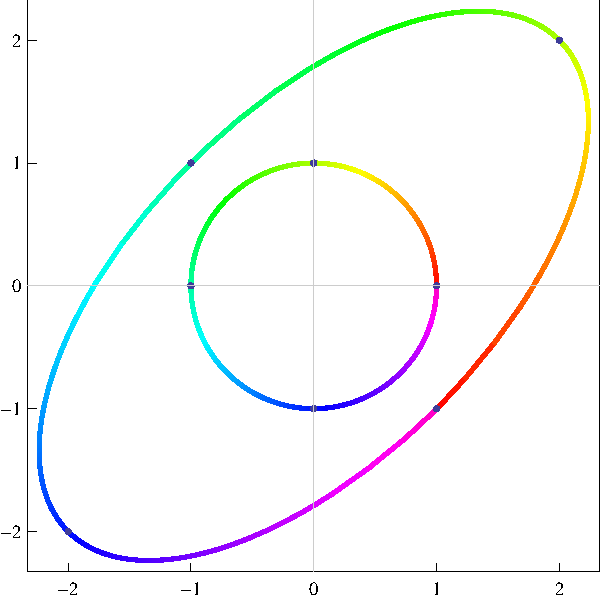
\includegraphics[ width = 2.5in ]{pdf/post_mortemII/dim_22_rank_2_image3} 
   \caption{The mapping action of the matrix in equation \eqref{eq:pmII:A} on all possible unit vectors in $\real{2}$. The coloring of the line is related to the angle. Fiducial marks are shown in increments of $\frac{\pi}{2}$.}
   \label{fig:maps:both}
\end{figure}

The next two plots, in figure \eqref{fig:maps:ev}, separate the curves and adds the eigenvectors. The black arrows are the first eigenvectors and the blue arrows are the second eigenvectors. The unit circle is resolved by the $\X{}$ matrix and the ellipse is resolved by the $\Y{}$ matrix \textit{scaled} by the singular values. This is codified in table \eqref{tab:pmII:blackblue}.

\begin{table}[htdp]
\begin{center}
\boxed{
\begin{tabular}{lrr}
  figure  & blue vector & black vector \\\hline
  circle  & $\X{}_{*,1}$\ \ \ \ \  & $\X{}_{*,2}$\ \ \ \ \  \\
  ellipse & $\sigma_{1} \Y{}_{*,1}$\ \ \ \ \  & $\sigma_{2} \Y{}_{*,2}$\ \ \ \ \ 
\end{tabular}
}
\end{center}
\label{tab:pmII:blackblue}
\caption{The eigenvectors of the domain and codomain and the scaling action of the eigenvectors.}
\end{table}%

This shows the vital relation between the column vectors of the domain and the scaled column vectors of the codomain:
\begin{equation}
  \A{} \X{}_{*,k} = \sigma_{k}\Y{}_{*,k}, \qquad k=1,\rho
  \label{eq:pmII:vital}
\end{equation}
This is of course just a rearrangement of the epitath
$$
\svdax{*}.
$$
The role of the singular values as scale factors is now clear after this demonstration. The blue vectors show the scaling effect of the first singular value; the black vectors the second singular value.

\begin{figure}[htbp] %  figure placement: here, top, bottom, or page
   \centering
   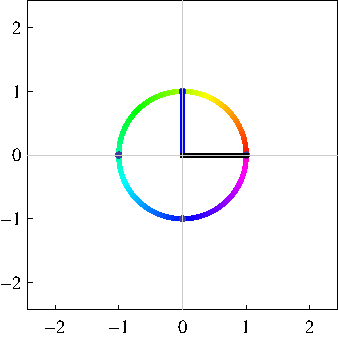
\includegraphics[ width = 2.25in ]{pdf/post_mortemII/circle_ev} \qquad
   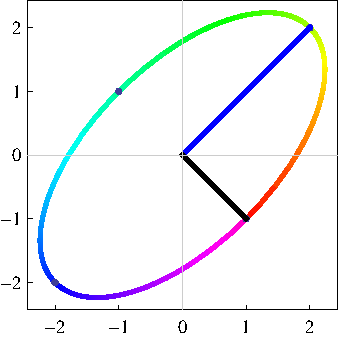
\includegraphics[ width = 2.25in ]{pdf/post_mortemII/ellipse_ev} 
   \caption{The pictorial demonstration of the scaling function of the singular values. The blue vectors show how $\A{} \X{}_{*,1} = \sigma_{k}\Y{}_{*,1}$ and the black vectors show $\A{} \X{}_{*,2} = \sigma_{2}\Y{}_{*,2}$.}
   \label{fig:maps:ev}
\end{figure}

%%
\subsection{The matrix in the simple method}
Look at the map in both directions

%%
\subsubsection{$\A{}x=y$}
\begin{figure}[htbp] %  figure placement: here, top, bottom, or page
   \centering
   \includegraphics[ ]{pdf/post_mortemII/toright} 
   \caption{Examine the mapping action of $\A{}$ from domain to codomain.}
   \label{fig:toright}
\end{figure}

The matrix described in equation \eqref{eq:simple:IamA}.
Recall the first decomposition \eqref{eq:simple:svd}
\begin{equation*}
  \begin{split}
    \svda{T} \\
    \Aexample &= \Yshade \Sigmaexampleb \Xtshade.
  \end{split}
\end{equation*}

Here the rank $\rho=1$ and so there is only one eigenvector to map. The eigenvector $\X{}_{*,1}$ maps to $\sigma_{1}\Y{}_{*,1}$. Since we can't distinctly see the mapping in the 3-dimensional image we show the explicit computation:
\begin{equation}
  \begin{split}
    \A{}\,\X{}_{*,1}\quad &= \quad \sigma_{1}\Y{}_{*,1}, \\
    \Aexample \frac{1}{\sqrt{2}}\mat{r}{1\\-1} \quad & =  \quad \sqrt{6}\frac{1}{\sqrt{3}}\mat{r}{1\\-1\\1}\\
    \frac{2}{\sqrt{2}}\mat{r}{1\\-1\\1}  \quad & =  \quad \sqrt{2}\mat{r}{1\\-1\\1}.
  \end{split}
\end{equation}

Herein lies the problem with the map. The dimension of the image, 1, is less than the dimension of the codomain, 3.

\begin{figure}[htbp] %  figure placement: here, top, bottom, or page
   \centering
   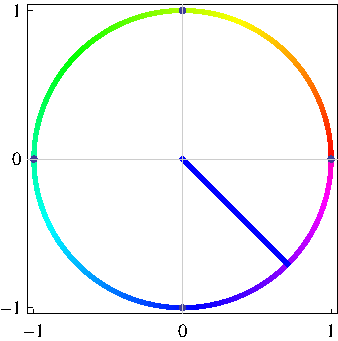
\includegraphics[ width = 1.9in ]{pdf/post_mortemII/a_circle_ev} \qquad
   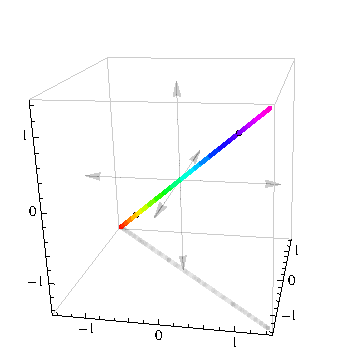
\includegraphics[ ]{pdf/post_mortemII/dim_32_rank_1_image} 
   \caption{The trouble with the matrix $\A{}$ (equation \eqref{eq:simple:IamA}) as a map from domain to codomain. The codomain has dimension 3 yet the image of the target matrix is a line with dimension 1. Because the line is embedded in a $3-$space a point on the line has three coordinates. But along the line there is only one coordinate measuring distance from the origin.}
   \label{fig:toright}
\end{figure}

%%
\subsubsection{$\A{T}y=x$}
\begin{figure}[htbp] %  figure placement: here, top, bottom, or page
   \centering
   \includegraphics[ ]{pdf/post_mortemII/toleft} 
   \caption{Examine the mapping action of the transpose matrix $\A{T}$ from codomain to domain.}
   \label{fig:toright}
\end{figure}
\begin{equation}
  \begin{split}
    \A{T} &= \svdt{T} \\
    \Atexample &= \Xshade \Sigmatexamplea \Ytshade.
  \end{split}
  \label{eq:simple:IamAT}
\end{equation}

\begin{equation}
  \begin{split}
    \A{}\,\X{}_{*,1}\quad &= \quad \sigma_{1}\Y{}_{*,1}, \\
    \Atexample \frac{1}{\sqrt{3}}\mat{r}{1\\-1\\1} \quad & =  \quad \sqrt{6}\frac{1}{\sqrt{2}}\mat{r}{1\\-1}\\
    \frac{3}{\sqrt{3}}\mat{r}{1\\-1}  \quad & =  \quad \sqrt{3}\mat{r}{1\\-1}.
  \end{split}
\end{equation}

\begin{figure}[htbp] %  figure placement: here, top, bottom, or page
   \centering
   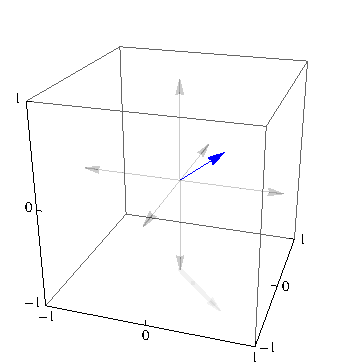
\includegraphics[ ]{pdf/post_mortemII/3_vector}  \qquad
   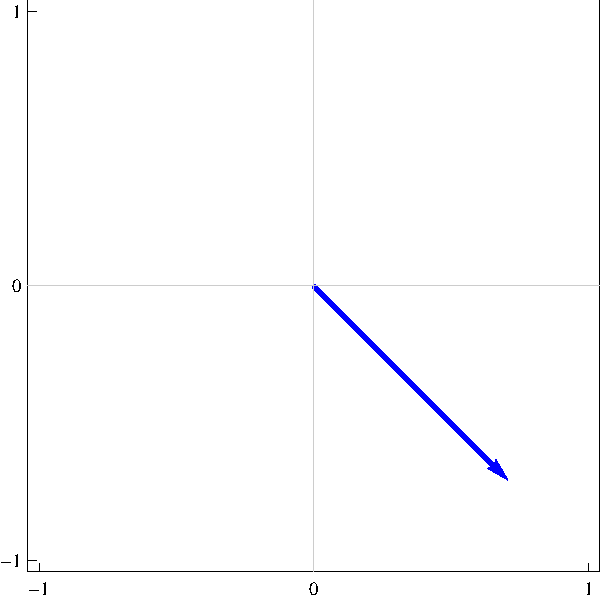
\includegraphics[ width = 1.9in ]{pdf/post_mortemII/430}
   \caption{The trouble with the matrix $\A{T}$ (equation \eqref{eq:simple:IamAT}) as a map from codomain to domain. The codomain has dimension 3 yet the image of the target matrix is a line with dimension 1. Because the line is embedded in a $2-$space a point on the line has two coordinates. But along the line there is only one coordinate measuring distance from the origin.}
   \label{fig:toleft}
\end{figure}

%%
\subsection{The matrix in the general method}
Look at the map in both directions

%%
\subsubsection{Domain $\longrightarrow$ cdomain}
\begin{figure}[htbp] %  figure placement: here, top, bottom, or page
   \centering
   \includegraphics[ ]{pdf/post_mortemII/toright} 
   \caption{Examine the mapping action of $\A{}$ from domain to codomain.}
   \label{fig:toright}
\end{figure}

Start with the first decomposition \eqref{eq:gen:soln}.
\begin{equation}
  \begin{split}
    \A{} &= \Y{}\paren{\sig{}\,\X{T}},\\
     &=
  \frac{1}{\sqrt{2}}
  \mat{rr}{1 & -1\\1 & 1}
  \frac{1}{\sqrt{2}}
  \paren{
  \mat{crc}
  {
  1 & 5  & 2 \\
  1 & -1 & 2
  }}, \\
  &=
  \mat{ccc}
  {
  0 & 3 & 0 \\
  1 & 2 & 2
  }.
  \end{split}
  \label{eq:gen:soln}
\end{equation}

Here the rank $\rho=1$ and so there is only one eigenvector to map. The eigenvector $\X{}_{*,1}$ maps to $\sigma_{1}\Y{}_{*,1}$. Since we can't distinctly see the mapping in the 3-dimensional image we show the explicit computation:
\begin{equation}
  \begin{split}
    \A{}\,\X{}_{*,1}\quad &= \quad \sigma_{1}\Y{}_{*,1}, \\
    \Aexample \frac{1}{\sqrt{2}}\mat{r}{1\\-1} \quad & =  \quad \sqrt{6}\frac{1}{\sqrt{3}}\mat{r}{1\\-1\\1}\\
    \frac{2}{\sqrt{2}}\mat{r}{1\\-1\\1}  \quad & =  \quad \sqrt{2}\mat{r}{1\\-1\\1}.
  \end{split}
\end{equation}

Herein lies the problem with the map. The dimension of the image, 1, is less than the dimension of the codomain, 3.

\begin{figure}[htbp] %  figure placement: here, top, bottom, or page
   \centering
   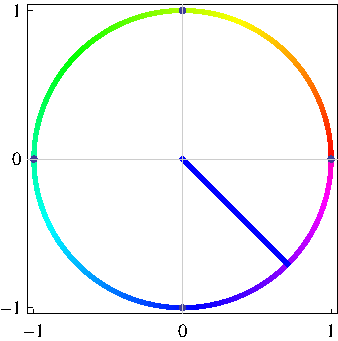
\includegraphics[ width = 1.9in ]{pdf/post_mortemII/a_circle_ev} \qquad
   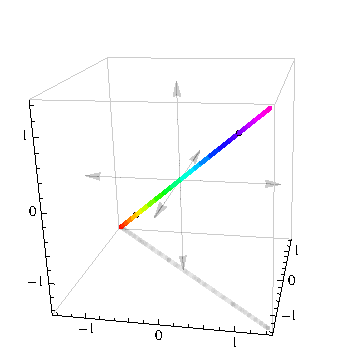
\includegraphics[ ]{pdf/post_mortemII/dim_32_rank_1_image} 
   \caption{The trouble with the matrix $\A{}$ (equation \eqref{eq:simple:IamA}) as a map from domain to codomain. The codomain has dimension 3 yet the image of the target matrix is a line with dimension 1. Because the line is embedded in a $3-$space a point on the line has three coordinates. But along the line there is only one coordinate measuring distance from the origin.}
   \label{fig:toright}
\end{figure}

%%
\subsubsection{$\A{T}y=x$}
\begin{figure}[htbp] %  figure placement: here, top, bottom, or page
   \centering
   \includegraphics[ ]{pdf/post_mortemII/toleft} 
   \caption{Examine the mapping action of the transpose matrix $\A{T}$ from codomain to domain.}
   \label{fig:toright}
\end{figure}
\begin{equation}
  \begin{split}
    \A{T} &= \svdt{T} \\
    \Atexample &= \Xshade \Sigmatexamplea \Ytshade.
  \end{split}
  \label{eq:simple:IamAT}
\end{equation}

\begin{equation}
  \begin{split}
    \A{}\,\X{}_{*,1}\quad &= \quad \sigma_{1}\Y{}_{*,1}, \\
    \Atexample \frac{1}{\sqrt{3}}\mat{r}{1\\-1\\1} \quad & =  \quad \sqrt{6}\,\frac{1}{\sqrt{2}}\mat{r}{1\\-1}\\
    \frac{3}{\sqrt{3}}\mat{r}{1\\-1}  \quad & =  \quad \sqrt{3}\mat{r}{1\\-1}.
  \end{split}
\end{equation}

\begin{figure}[htbp] %  figure placement: here, top, bottom, or page
   \centering
   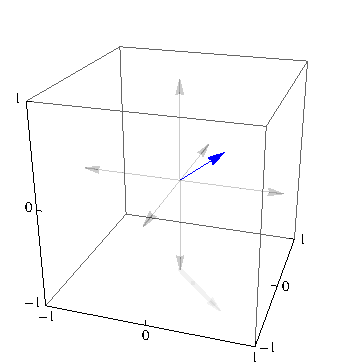
\includegraphics[ ]{pdf/post_mortemII/3_vector}  \qquad
   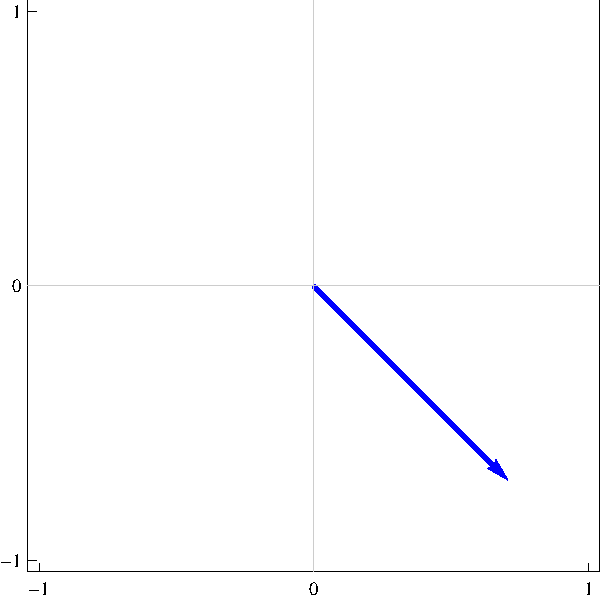
\includegraphics[ width = 1.9in ]{pdf/post_mortemII/430}
   \caption{The trouble with the matrix $\A{T}$ (equation \eqref{eq:simple:IamAT}) as a map from codomain to domain. The codomain has dimension 3 yet the image of the target matrix is a line with dimension 1. Because the line is embedded in a $2-$space a point on the line has two coordinates. But along the line there is only one coordinate measuring distance from the origin.}
   \label{fig:toleft}
\end{figure}


\endinput
\section{A survey of matrix mappings}
In the following pages we will look at three different kinds of mappings for a matrix $\Acc{m}{n}$: no frustration, frustration in one direction, frustration in both directions.

There are two different ways to view frustrated\index{frustration} mappings:
\begin{enumerate}
\item geometric deficiency\index{geometric deficiency} - mapping into a lower dimensional object;
\item algebraic deficiency\index{algebraic deficiency} - rank deficiency in row or column.
\end{enumerate}

In the examples that follow we will see ellipses mapped into other ellipses. These mappings are not frustrated. But once we map into a lower dimensional object, say from the unit sphere onto a line, the map is frustrated. This also means that we can't reverse the map. We can't make a finite linear map from a line with one parameter onto a sphere with three parameters.

These tables specify critical properties of the target matrix.

\textbf{Plots: }All plots start with the unit circle which is either
\begin{equation}
  \begin{array}{rcll}
     S(\theta) &=& \mat{c}{\cos \theta\\\sin \theta},\ \theta\in[0,2\pi) \qquad &n=2,\\
     S(\theta,\phi) &=& \mat{c}{\cos \theta\sin \phi\\\sin \theta \sin \phi\\\cos \phi},\ \theta\in[0,2\pi),\ \phi\in[0,\pi), \qquad &n=3.
  \end{array}
\end{equation}
Then look at the mapping action of the matrix. The result is either
\begin{equation}
  \A{}S(\theta) 
\end{equation}
when the target matrix has two columns or
\begin{equation}
  \A{}S(\theta,\phi) 
\end{equation}
when the target matrix has three columns.

The circles and ellipses have the color determined the the angular variable to provide an clearer idea of how the unit circle is distorted. So for the color red starts at $\theta=0$ and progresses through the spectrum until $\theta=2pi$ where the color is violet.\\

\textbf{Matrix images:} This block summarizes the plot above. For example, it may say that the plot represents a unit sphere being mapped to a line.\\

%%
\textbf{Vector space mappings:} These mappings are based on the dimensions of the spaces for the row and column vectors, $m$ and $n$. They disregard the issue of rank and and concerned purely with the mappings $\real{m}\mapsto\real{n}$ and  $\real{n}\mapsto\real{m}$. This map addresses the geometric deficiency of the mappings. For example are we going from a plane to a plane or a plane to a line. If the map is into a higher dimensional space we will have a frustrated map.\\

\textbf{Matrix ranks:} Are there rank deficiencies in the row or column space? If there is a rank deficiency we will see a frustrated map. 


\clearpage

%%
%% 2 x 2
%%
\begin{table}[htdp]
\begin{center}
\begin{tabular}{cc}
  $\A{}x=y$ & $\A{T}y=x$\\
 $\textellipsis$ & $\textellipsis$ \\
$\mat{rr}{1&2\\-1&2}\mat{c}{x_{1}\\x_{2}} = \mat{c}{y_{1}\\y_{2}}$ &
$\mat{rr}{1&-1\\2&2}\mat{c}{x_{1}\\x_{2}} = \mat{c}{y_{1}\\y_{2}}$ \\
\ \\
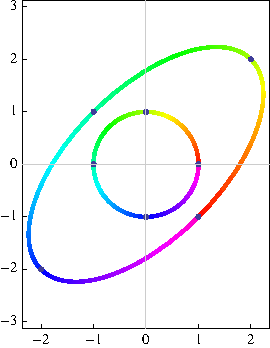
\includegraphics[ width = 2.15in ]{pdf/post_mortemII/2_2_2} &
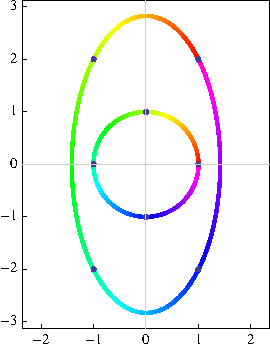
\includegraphics[ width = 2.15in ]{pdf/post_mortemII/2_2_2_t} \\
%%
\ \\
 matrix image & transpose matrix image \\
unit circle $\mapsto$ ellipse & unit circle $\mapsto$ ellipse\\
 $\textellipsis$ & $\textellipsis$ \\
vector space mappings & vector space mappings\\
(Domain) $\real{2} \mapsto \real{2}$ (Codomain) & (Codomain) $\real{2} \mapsto \real{2}$ (Domain)\\
 $\textellipsis$ & $\textellipsis$ \\
 full column rank  & full row rank\\
  $\textellipsis$ & $\textellipsis$ \\
 $\Ap=\AinvL$ & $\Ap=\AinvR$\\[10pt]
\end{tabular}
\end{center}
\label{tab:interpII:a}
\caption{Maps with no frustration. The domain and the codomain have the same dimension and the matrix has full rank. There are no null spaces associated with either the matrix or its transpose. The block dots are fiducial marks to help with comparing the orientation of the image (ellipse) relative to the target (circle). This matrix has full row rank, therefore the pseudoinverse is a left inverse. This matrix has full column rank, therefore the pseudoinverse is a right inverse. Because the pseudoinverse is both a left and a right inverse the pseudoinverse is also the standard inverse.}
\end{table}%

\clearpage
%%
%% 2 x 3
%%
\begin{table}[htdp]
\begin{center}
\begin{tabular}{cc}
  $\A{}x=y$ & $\A{T}y=x$\\
 $\textellipsis$ & $\textellipsis$ \\
$\mat{ccc}{0&3&0\\1&1&2}\mat{c}{x_{1}\\x_{2}\\x_{3}} = \mat{c}{y_{1}\\y_{2}}$ &
$\mat{cc}{0&1\\3&1\\0&2}\mat{c}{y_{1}\\y_{2}} = \mat{c}{x_{1}\\x_{2}\\x_{3}}$ \\
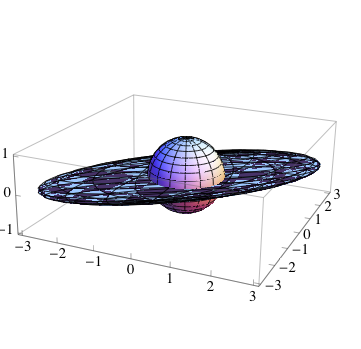
\includegraphics[ width = 2.5in ]{pdf/post_mortemII/3_2_2.png} &
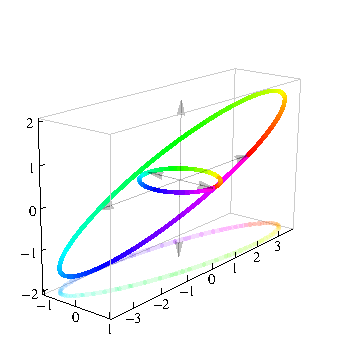
\includegraphics[ width = 2.5in ]{pdf/post_mortemII/3_2_2_t} \\
%%
vector space mappings & vector space mappings\\
(Domain) $\real{3} \mapsto \real{2}$ (Codomain) & (Codomain) $\real{2} \mapsto \real{3}$ (Domain)\\
 $\textellipsis$ & $\textellipsis$ \\
 matrix image & transpose matrix image \\
unit sphere $\mapsto$ elliptic disk & unit circle $\mapsto$ ellipse\\
 $\textellipsis$ & $\textellipsis$ \\
column rank deficient & full row rank\\
frustrated map\\
 $\textellipsis$ & $\textellipsis$ \\
 $\nexists\ \AinvL$ & $\Ap=\AinvR$\\[10pt]
\end{tabular}
\end{center}
\label{tab:interpII:a}
\caption{Frustration in one direction: domain to codomain. The frustration is signaled by the column rank deficiency where the matrix rank is less than the number of columns $(\rho<n)$. Notice that the mapping on the right is not frustrated; it is from a circle to an ellipse. Although both are two-dimensional objects, the ellipse is tipped and tilted out of the plane. The floor of the figure shows a shadow of the ellipse which helps to visualize the orientation in three-space. Because the matrix has full column rank the pseudoinverse is a right inverse.}
\end{table}

\clearpage
%%
%% 3 x 2
%%
\begin{table}[htdp]
\begin{center}
\begin{tabular}{cc}
  $\A{}x=y$ & $\A{T}y=x$\\
 $\textellipsis$ & $\textellipsis$ \\
$\Aexample \mat{c}{x_{1}\\x_{2}} = \mat{c}{y_{1}\\y_{2}\\y_{3}}$ &
$\Atexample\mat{c}{x_{1}\\x_{2}\\x_{3}} = \mat{c}{y_{1}\\y_{2}}$ \\
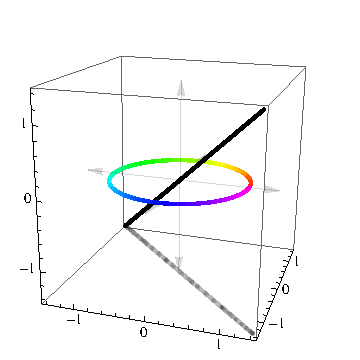
\includegraphics[ width = 2.5in ]{pdf/post_mortemII/3_2_1_a} &
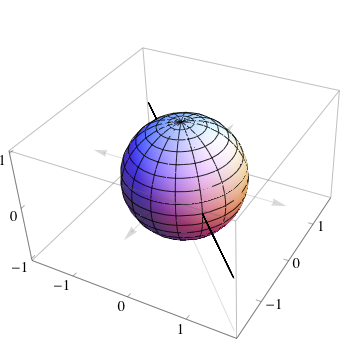
\includegraphics[ width = 2.5in ]{pdf/post_mortemII/3_2_1_t_a} \\
%%
vector space mappings & vector space mappings\\
(Domain) $\real{2} \mapsto \real{3}$ (Codomain) & (Codomain) $\real{3} \mapsto \real{2}$ (Domain)\\
 $\textellipsis$ & $\textellipsis$ \\
 matrix image & transpose matrix image \\
unit circle $\mapsto$ line & unit sphere $\mapsto$ line\\
 $\textellipsis$ & $\textellipsis$ \\
column rank deficient & row rank deficient\\
frustrated map & frustrated map\\
 $\textellipsis$ & $\textellipsis$ \\
 $\nexists\ \AinvL$ &  $\nexists\ \AinvR$ \\[10pt]
\end{tabular}
\end{center}
\label{tab:interpII:c}
\caption{Frustration in both directions, domain to codomain and back. The matrix rank is less than the number of rows $(\rho<m)$ and less than the number of columns $(\rho<n)$. The line is shown in black because the mapping is not one-to-one; multiple points in the target map to the same point in the image. Both figures show a projection of the image onto the floor of the figure. Because the matrix is both column and rank deficient there is neither a left nor a right inverse.}
\end{table}

\endinput



\endinput